\subsubsection{Zabrak}
\begin{samepage}
	\begin{flushright}
		\begin{tabular}{ l l }
			\textbf{Type} 			& Humanoïde \\
		   	\textbf{Planète} 		& Iridonia \\
		   	\textbf{Language} 		& Zabraki \\
		   	\textbf{Orientation} 	& Obscur \\
		\end{tabular}
	\end{flushright}
	\vspace{-6\baselineskip}
	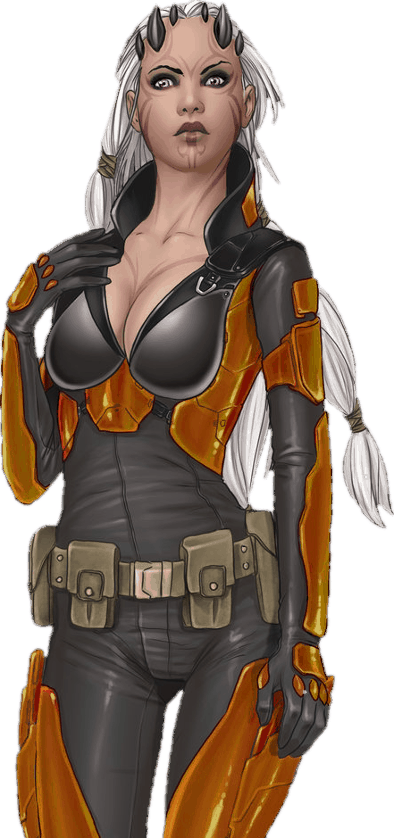
\includegraphics[width=5cm]{img/races/zabrak.png}
\end{samepage}

Originaires de la planète Iridonia, les Zabraks sont des humanoïdes d'une taille pouvant aller de 1,60 mètre à 2,10 mètres, et dont la tête était recouverte de petites cornes et le corps de tatouages, qui donnent à cette espèce un aspect parfois effrayant. Très tôt dans l'histoire galactique les Zabraks ont atteint un niveau de technologie élevé et ont pu coloniser plusieurs mondes extérieurs aux alentours de leur planète natale. On estime que cette espèce a ainsi établi huit colonies dans la Bordure Extérieure, et que les différents groupes coloniaux ont pu prospérer de façon suffisamment importante pour que les Zabraks s'identifient eux-même selon les colonies d'où ils viennent, plutôt que par rapport à Iridonia uniquement.

---

Les Zabraks dans leur ensemble possèdent un fort caractère et une volonté de fer, doublé d'un instinct de survie supérieur à la plupart des autres espèces.

Ce sont des explorateurs courageux et des guerriers que rien n'effraie.


\begin{description}[align=left]
\item [Force de la nature] 				% CAP +2
	L'imagerie populaire veut que les Wookies soit physiquement la race la plus forte de la galaxie (en tous cas, par rapport à sa taille).\\
	\emph{d6 For}
\item [Increvable] 						% CAP +2 +3
	Les Wookies possèdent, entres autres, de remarquables capacités de récupération, et sont capables de survivre à des blessures très graves.\\
	\emph{Increvable}\\
	\emph{Combatif}
\item [Shyriiwook] 						% CAP -1
		Les Wookies parlent entre eux leur langage, le Shyriiwook, un dialecte très complexe, en raison du mélange de feulements, rugissements, gestes et autres bruits nécessaires à son usage.\\
		\emph{Ne parle pas le Basic}
\item [Force \& Honneur] 				% CAP -2
	Comme de nombreux peuples mettant en avant des valeurs comme l'honneur, les Wookies pratiquent les serments et la "dette de vie". Celle-ci peut les amener à défendre jusqu'à la mort un étranger (même d'une autre race) auquel ils pensent devoir une grande faveur. Une dette de vie est définitive et rien ne peut la lever.\\
	\emph{Code d'honneur}
\item [Ennemis jurés] 					% CAP -1
	Les ennemis jurés des Wookies, les Trandoshans, se firent à cette époque un malin plaisir à chasser et à capturer les wookies.\\
	\emph{Ennemi Racial (Trandoshans) -4 Cha}
\item [Il faut partir à point] 			% CAP -1
	De par leur stature, les Wookies ne sont pas les êtres les plus vif de la galaxy.\\
	\emph{Allure 5}
\end{description}